% Options for packages loaded elsewhere
\PassOptionsToPackage{unicode}{hyperref}
\PassOptionsToPackage{hyphens}{url}
\PassOptionsToPackage{dvipsnames,svgnames,x11names}{xcolor}
%
\documentclass[
  letterpaper,
  DIV=11,
  numbers=noendperiod]{scrartcl}

\usepackage{amsmath,amssymb}
\usepackage{iftex}
\ifPDFTeX
  \usepackage[T1]{fontenc}
  \usepackage[utf8]{inputenc}
  \usepackage{textcomp} % provide euro and other symbols
\else % if luatex or xetex
  \usepackage{unicode-math}
  \defaultfontfeatures{Scale=MatchLowercase}
  \defaultfontfeatures[\rmfamily]{Ligatures=TeX,Scale=1}
\fi
\usepackage{lmodern}
\ifPDFTeX\else  
    % xetex/luatex font selection
\fi
% Use upquote if available, for straight quotes in verbatim environments
\IfFileExists{upquote.sty}{\usepackage{upquote}}{}
\IfFileExists{microtype.sty}{% use microtype if available
  \usepackage[]{microtype}
  \UseMicrotypeSet[protrusion]{basicmath} % disable protrusion for tt fonts
}{}
\makeatletter
\@ifundefined{KOMAClassName}{% if non-KOMA class
  \IfFileExists{parskip.sty}{%
    \usepackage{parskip}
  }{% else
    \setlength{\parindent}{0pt}
    \setlength{\parskip}{6pt plus 2pt minus 1pt}}
}{% if KOMA class
  \KOMAoptions{parskip=half}}
\makeatother
\usepackage{xcolor}
\setlength{\emergencystretch}{3em} % prevent overfull lines
\setcounter{secnumdepth}{-\maxdimen} % remove section numbering
% Make \paragraph and \subparagraph free-standing
\ifx\paragraph\undefined\else
  \let\oldparagraph\paragraph
  \renewcommand{\paragraph}[1]{\oldparagraph{#1}\mbox{}}
\fi
\ifx\subparagraph\undefined\else
  \let\oldsubparagraph\subparagraph
  \renewcommand{\subparagraph}[1]{\oldsubparagraph{#1}\mbox{}}
\fi

\usepackage{color}
\usepackage{fancyvrb}
\newcommand{\VerbBar}{|}
\newcommand{\VERB}{\Verb[commandchars=\\\{\}]}
\DefineVerbatimEnvironment{Highlighting}{Verbatim}{commandchars=\\\{\}}
% Add ',fontsize=\small' for more characters per line
\usepackage{framed}
\definecolor{shadecolor}{RGB}{241,243,245}
\newenvironment{Shaded}{\begin{snugshade}}{\end{snugshade}}
\newcommand{\AlertTok}[1]{\textcolor[rgb]{0.68,0.00,0.00}{#1}}
\newcommand{\AnnotationTok}[1]{\textcolor[rgb]{0.37,0.37,0.37}{#1}}
\newcommand{\AttributeTok}[1]{\textcolor[rgb]{0.40,0.45,0.13}{#1}}
\newcommand{\BaseNTok}[1]{\textcolor[rgb]{0.68,0.00,0.00}{#1}}
\newcommand{\BuiltInTok}[1]{\textcolor[rgb]{0.00,0.23,0.31}{#1}}
\newcommand{\CharTok}[1]{\textcolor[rgb]{0.13,0.47,0.30}{#1}}
\newcommand{\CommentTok}[1]{\textcolor[rgb]{0.37,0.37,0.37}{#1}}
\newcommand{\CommentVarTok}[1]{\textcolor[rgb]{0.37,0.37,0.37}{\textit{#1}}}
\newcommand{\ConstantTok}[1]{\textcolor[rgb]{0.56,0.35,0.01}{#1}}
\newcommand{\ControlFlowTok}[1]{\textcolor[rgb]{0.00,0.23,0.31}{#1}}
\newcommand{\DataTypeTok}[1]{\textcolor[rgb]{0.68,0.00,0.00}{#1}}
\newcommand{\DecValTok}[1]{\textcolor[rgb]{0.68,0.00,0.00}{#1}}
\newcommand{\DocumentationTok}[1]{\textcolor[rgb]{0.37,0.37,0.37}{\textit{#1}}}
\newcommand{\ErrorTok}[1]{\textcolor[rgb]{0.68,0.00,0.00}{#1}}
\newcommand{\ExtensionTok}[1]{\textcolor[rgb]{0.00,0.23,0.31}{#1}}
\newcommand{\FloatTok}[1]{\textcolor[rgb]{0.68,0.00,0.00}{#1}}
\newcommand{\FunctionTok}[1]{\textcolor[rgb]{0.28,0.35,0.67}{#1}}
\newcommand{\ImportTok}[1]{\textcolor[rgb]{0.00,0.46,0.62}{#1}}
\newcommand{\InformationTok}[1]{\textcolor[rgb]{0.37,0.37,0.37}{#1}}
\newcommand{\KeywordTok}[1]{\textcolor[rgb]{0.00,0.23,0.31}{#1}}
\newcommand{\NormalTok}[1]{\textcolor[rgb]{0.00,0.23,0.31}{#1}}
\newcommand{\OperatorTok}[1]{\textcolor[rgb]{0.37,0.37,0.37}{#1}}
\newcommand{\OtherTok}[1]{\textcolor[rgb]{0.00,0.23,0.31}{#1}}
\newcommand{\PreprocessorTok}[1]{\textcolor[rgb]{0.68,0.00,0.00}{#1}}
\newcommand{\RegionMarkerTok}[1]{\textcolor[rgb]{0.00,0.23,0.31}{#1}}
\newcommand{\SpecialCharTok}[1]{\textcolor[rgb]{0.37,0.37,0.37}{#1}}
\newcommand{\SpecialStringTok}[1]{\textcolor[rgb]{0.13,0.47,0.30}{#1}}
\newcommand{\StringTok}[1]{\textcolor[rgb]{0.13,0.47,0.30}{#1}}
\newcommand{\VariableTok}[1]{\textcolor[rgb]{0.07,0.07,0.07}{#1}}
\newcommand{\VerbatimStringTok}[1]{\textcolor[rgb]{0.13,0.47,0.30}{#1}}
\newcommand{\WarningTok}[1]{\textcolor[rgb]{0.37,0.37,0.37}{\textit{#1}}}

\providecommand{\tightlist}{%
  \setlength{\itemsep}{0pt}\setlength{\parskip}{0pt}}\usepackage{longtable,booktabs,array}
\usepackage{calc} % for calculating minipage widths
% Correct order of tables after \paragraph or \subparagraph
\usepackage{etoolbox}
\makeatletter
\patchcmd\longtable{\par}{\if@noskipsec\mbox{}\fi\par}{}{}
\makeatother
% Allow footnotes in longtable head/foot
\IfFileExists{footnotehyper.sty}{\usepackage{footnotehyper}}{\usepackage{footnote}}
\makesavenoteenv{longtable}
\usepackage{graphicx}
\makeatletter
\def\maxwidth{\ifdim\Gin@nat@width>\linewidth\linewidth\else\Gin@nat@width\fi}
\def\maxheight{\ifdim\Gin@nat@height>\textheight\textheight\else\Gin@nat@height\fi}
\makeatother
% Scale images if necessary, so that they will not overflow the page
% margins by default, and it is still possible to overwrite the defaults
% using explicit options in \includegraphics[width, height, ...]{}
\setkeys{Gin}{width=\maxwidth,height=\maxheight,keepaspectratio}
% Set default figure placement to htbp
\makeatletter
\def\fps@figure{htbp}
\makeatother

\KOMAoption{captions}{tableheading}
\makeatletter
\makeatother
\makeatletter
\makeatother
\makeatletter
\@ifpackageloaded{caption}{}{\usepackage{caption}}
\AtBeginDocument{%
\ifdefined\contentsname
  \renewcommand*\contentsname{Table of contents}
\else
  \newcommand\contentsname{Table of contents}
\fi
\ifdefined\listfigurename
  \renewcommand*\listfigurename{List of Figures}
\else
  \newcommand\listfigurename{List of Figures}
\fi
\ifdefined\listtablename
  \renewcommand*\listtablename{List of Tables}
\else
  \newcommand\listtablename{List of Tables}
\fi
\ifdefined\figurename
  \renewcommand*\figurename{Figure}
\else
  \newcommand\figurename{Figure}
\fi
\ifdefined\tablename
  \renewcommand*\tablename{Table}
\else
  \newcommand\tablename{Table}
\fi
}
\@ifpackageloaded{float}{}{\usepackage{float}}
\floatstyle{ruled}
\@ifundefined{c@chapter}{\newfloat{codelisting}{h}{lop}}{\newfloat{codelisting}{h}{lop}[chapter]}
\floatname{codelisting}{Listing}
\newcommand*\listoflistings{\listof{codelisting}{List of Listings}}
\makeatother
\makeatletter
\@ifpackageloaded{caption}{}{\usepackage{caption}}
\@ifpackageloaded{subcaption}{}{\usepackage{subcaption}}
\makeatother
\makeatletter
\@ifpackageloaded{tcolorbox}{}{\usepackage[skins,breakable]{tcolorbox}}
\makeatother
\makeatletter
\@ifundefined{shadecolor}{\definecolor{shadecolor}{rgb}{.97, .97, .97}}
\makeatother
\makeatletter
\makeatother
\makeatletter
\makeatother
\ifLuaTeX
  \usepackage{selnolig}  % disable illegal ligatures
\fi
\IfFileExists{bookmark.sty}{\usepackage{bookmark}}{\usepackage{hyperref}}
\IfFileExists{xurl.sty}{\usepackage{xurl}}{} % add URL line breaks if available
\urlstyle{same} % disable monospaced font for URLs
\hypersetup{
  pdftitle={TP1 (FAS 1001)},
  pdfauthor={Olivia Saffioti},
  colorlinks=true,
  linkcolor={blue},
  filecolor={Maroon},
  citecolor={Blue},
  urlcolor={Blue},
  pdfcreator={LaTeX via pandoc}}

\title{TP1 (FAS 1001)}
\author{Olivia Saffioti}
\date{2024-01-22}

\begin{document}
\maketitle
\ifdefined\Shaded\renewenvironment{Shaded}{\begin{tcolorbox}[boxrule=0pt, enhanced, sharp corners, breakable, interior hidden, frame hidden, borderline west={3pt}{0pt}{shadecolor}]}{\end{tcolorbox}}\fi

\begin{center}\rule{0.5\linewidth}{0.5pt}\end{center}

\hypertarget{quarto}{%
\subsection{Quarto}\label{quarto}}

Quarto enables you to weave together content and executable code into a
finished document. To learn more about Quarto see
\url{https://quarto.org}.

\hypertarget{running-code}{%
\subsection{Running Code}\label{running-code}}

When you click the \textbf{Render} button a document will be generated
that includes both content and the output of embedded code. You can
embed code like this:

You can add options to executable code like this

\begin{Shaded}
\begin{Highlighting}[]

\NormalTok{\textless{}\textless{}\textless{}\textless{}\textless{}\textless{}\textless{} HEAD}
\NormalTok{=======}

\NormalTok{\textgreater{}\textgreater{}\textgreater{}\textgreater{}\textgreater{}\textgreater{}\textgreater{} c3f3b4f (Images 2)}
\end{Highlighting}
\end{Shaded}

The \texttt{echo:\ false} option disables the printing of code (only
output is displayed).

\hypertarget{description-des-codes-git-utilisuxe9s}{%
\section{Description des codes Git
utilisés}\label{description-des-codes-git-utilisuxe9s}}

\hypertarget{images}{%
\subsection{Images :}\label{images}}

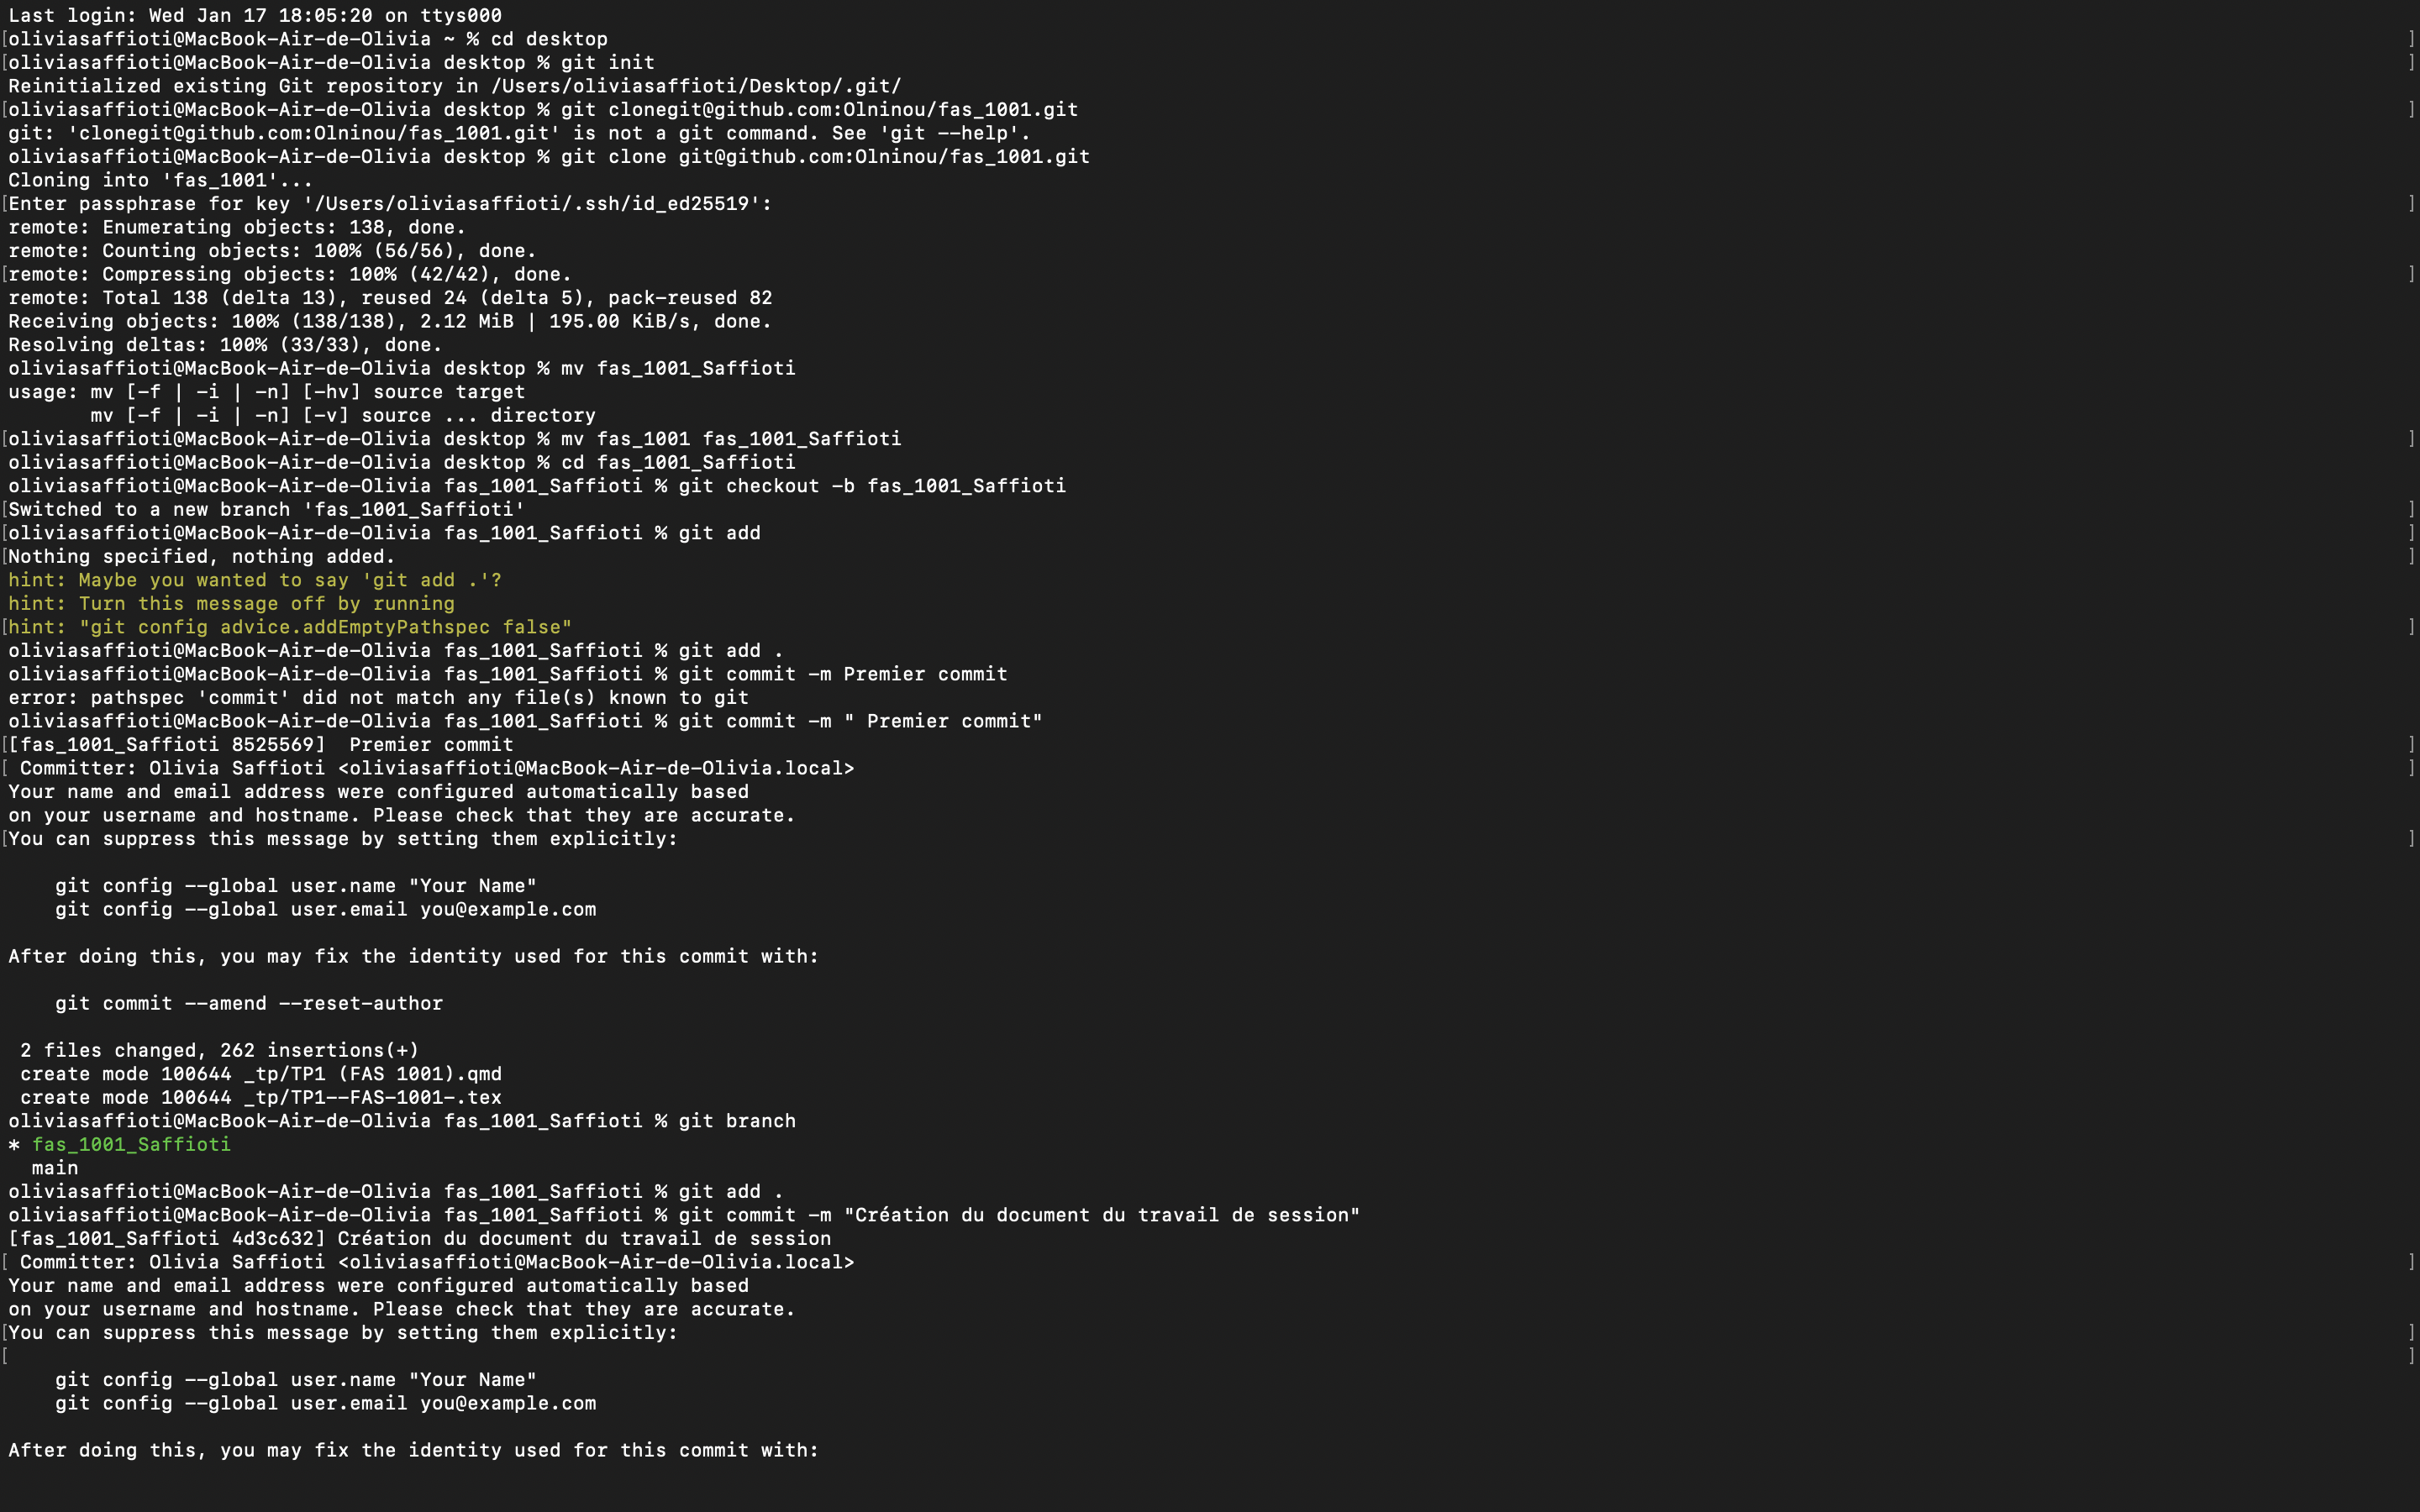
\includegraphics{//Users/oliviasaffioti/Desktop/fas_1001_Saffioti/_tp/Codes Git 1.png}
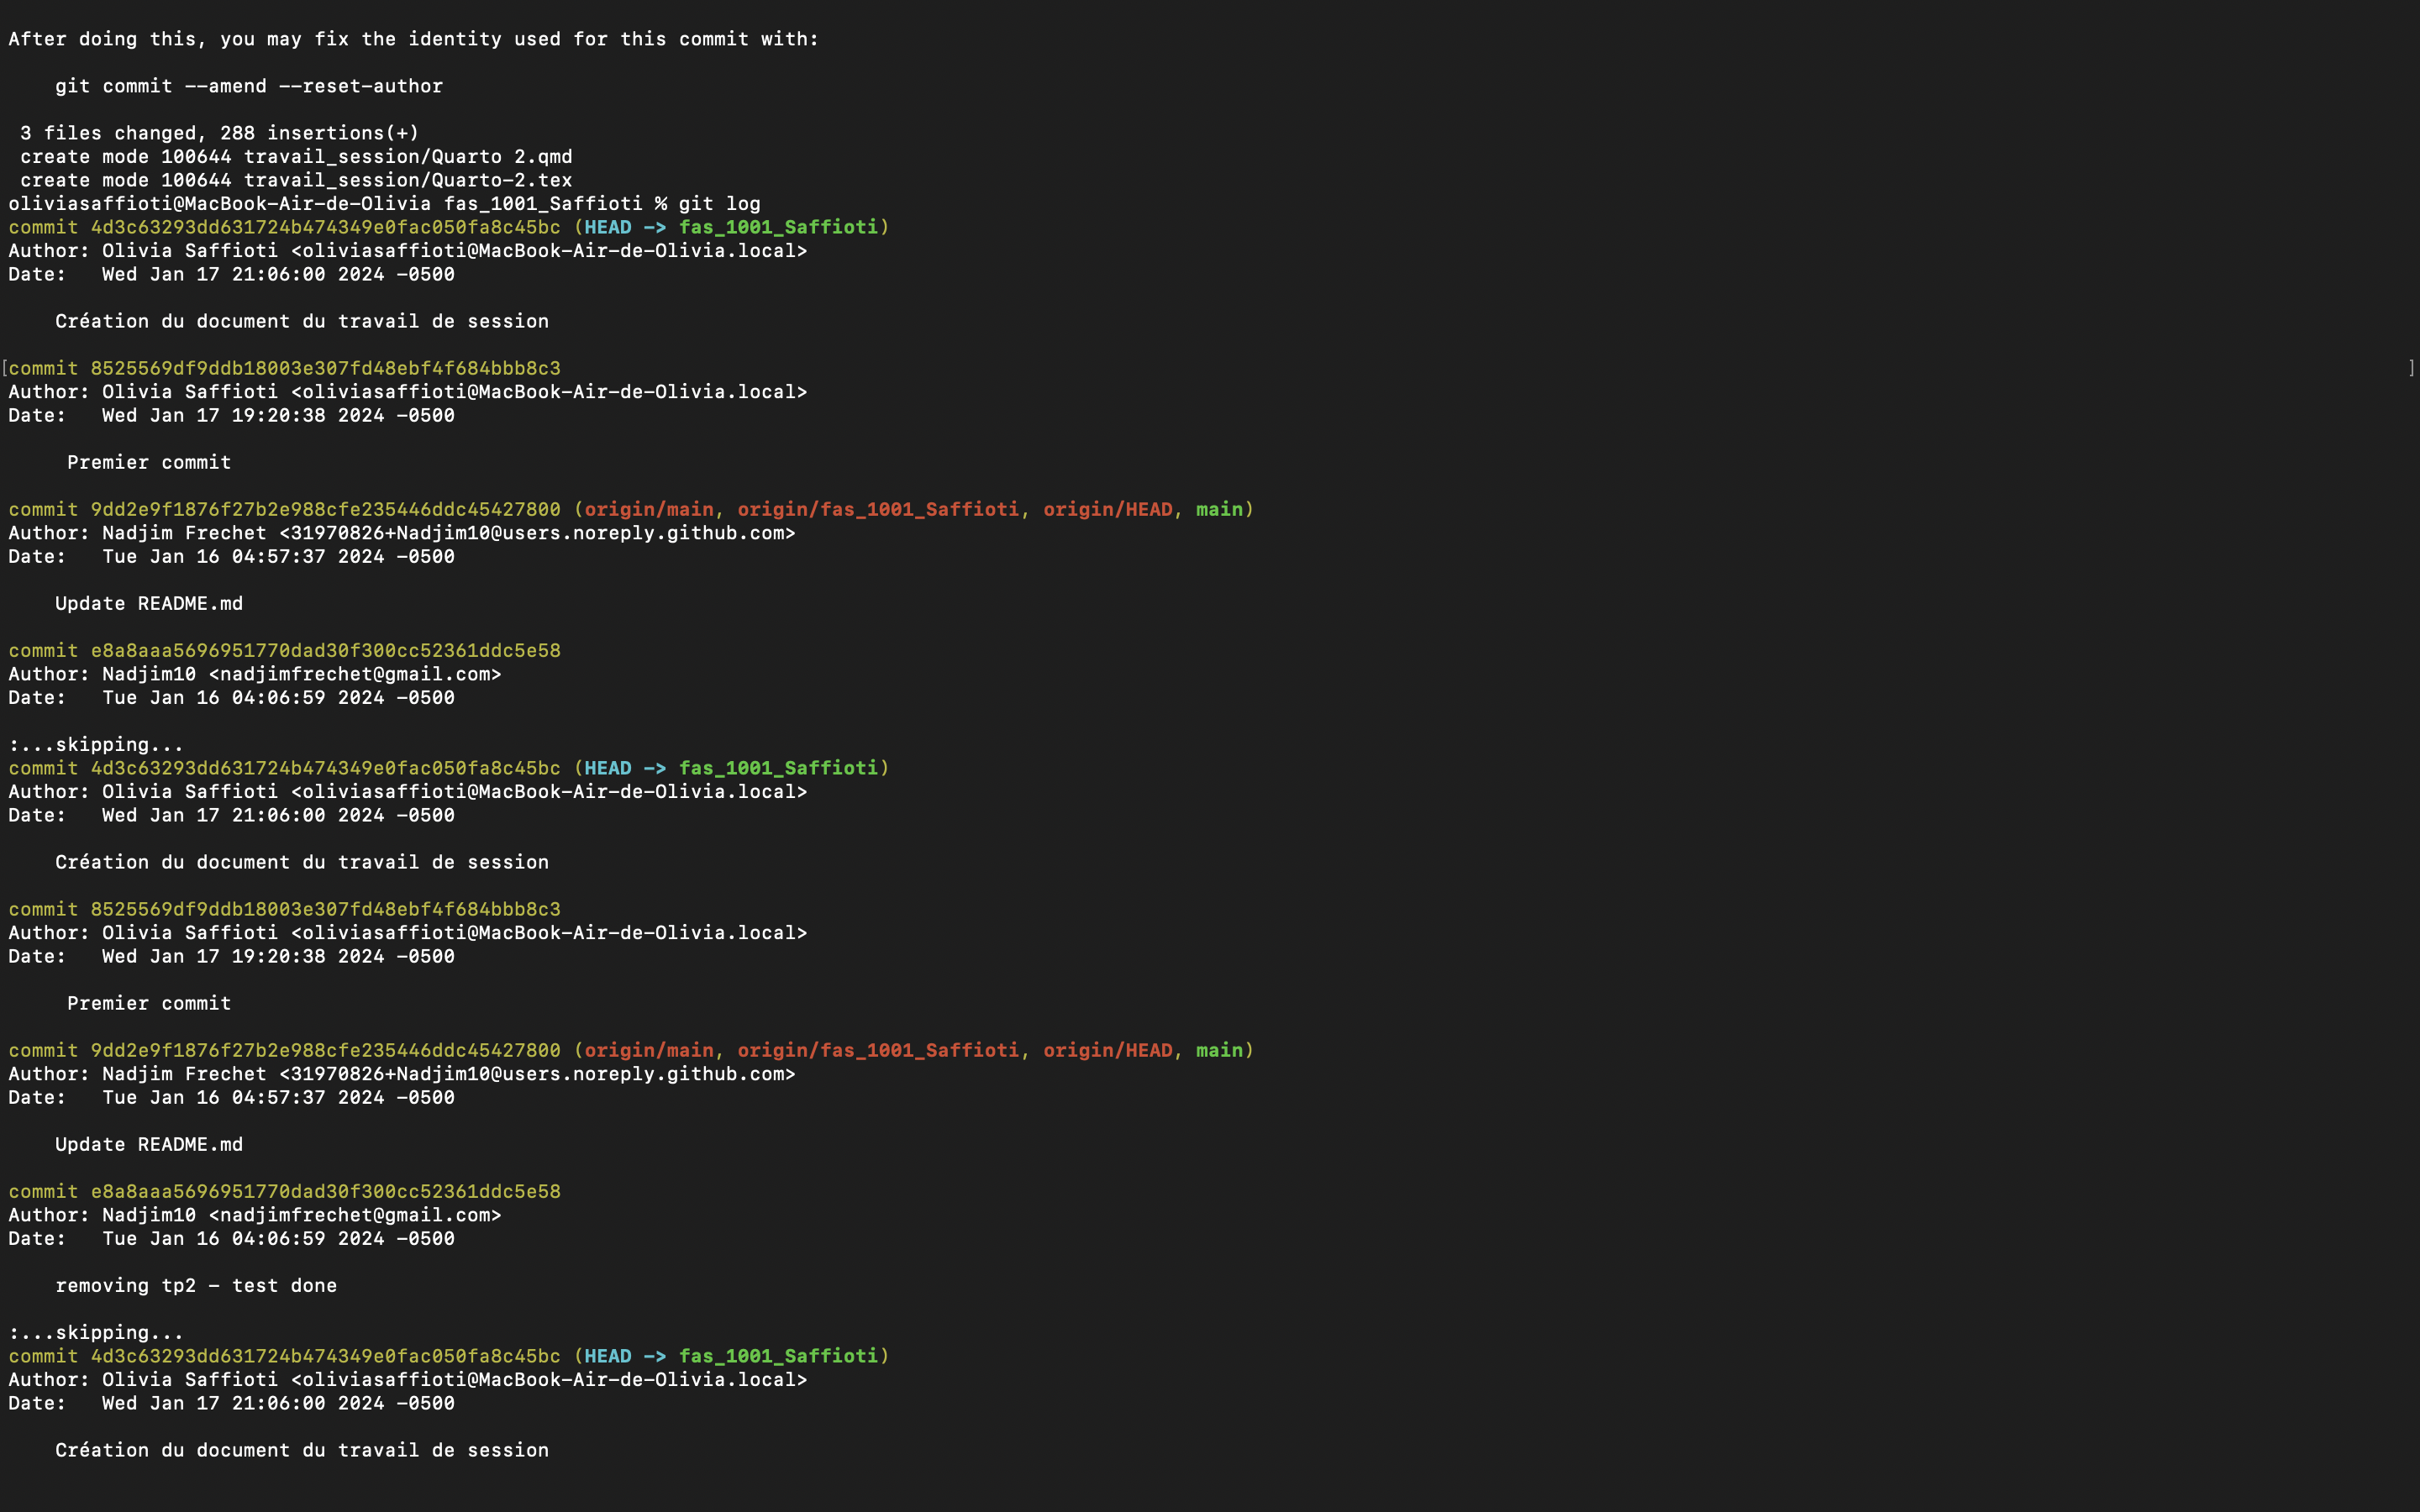
\includegraphics{//Users/oliviasaffioti/Desktop/fas_1001_Saffioti/_tp/Codes Git 2.png}
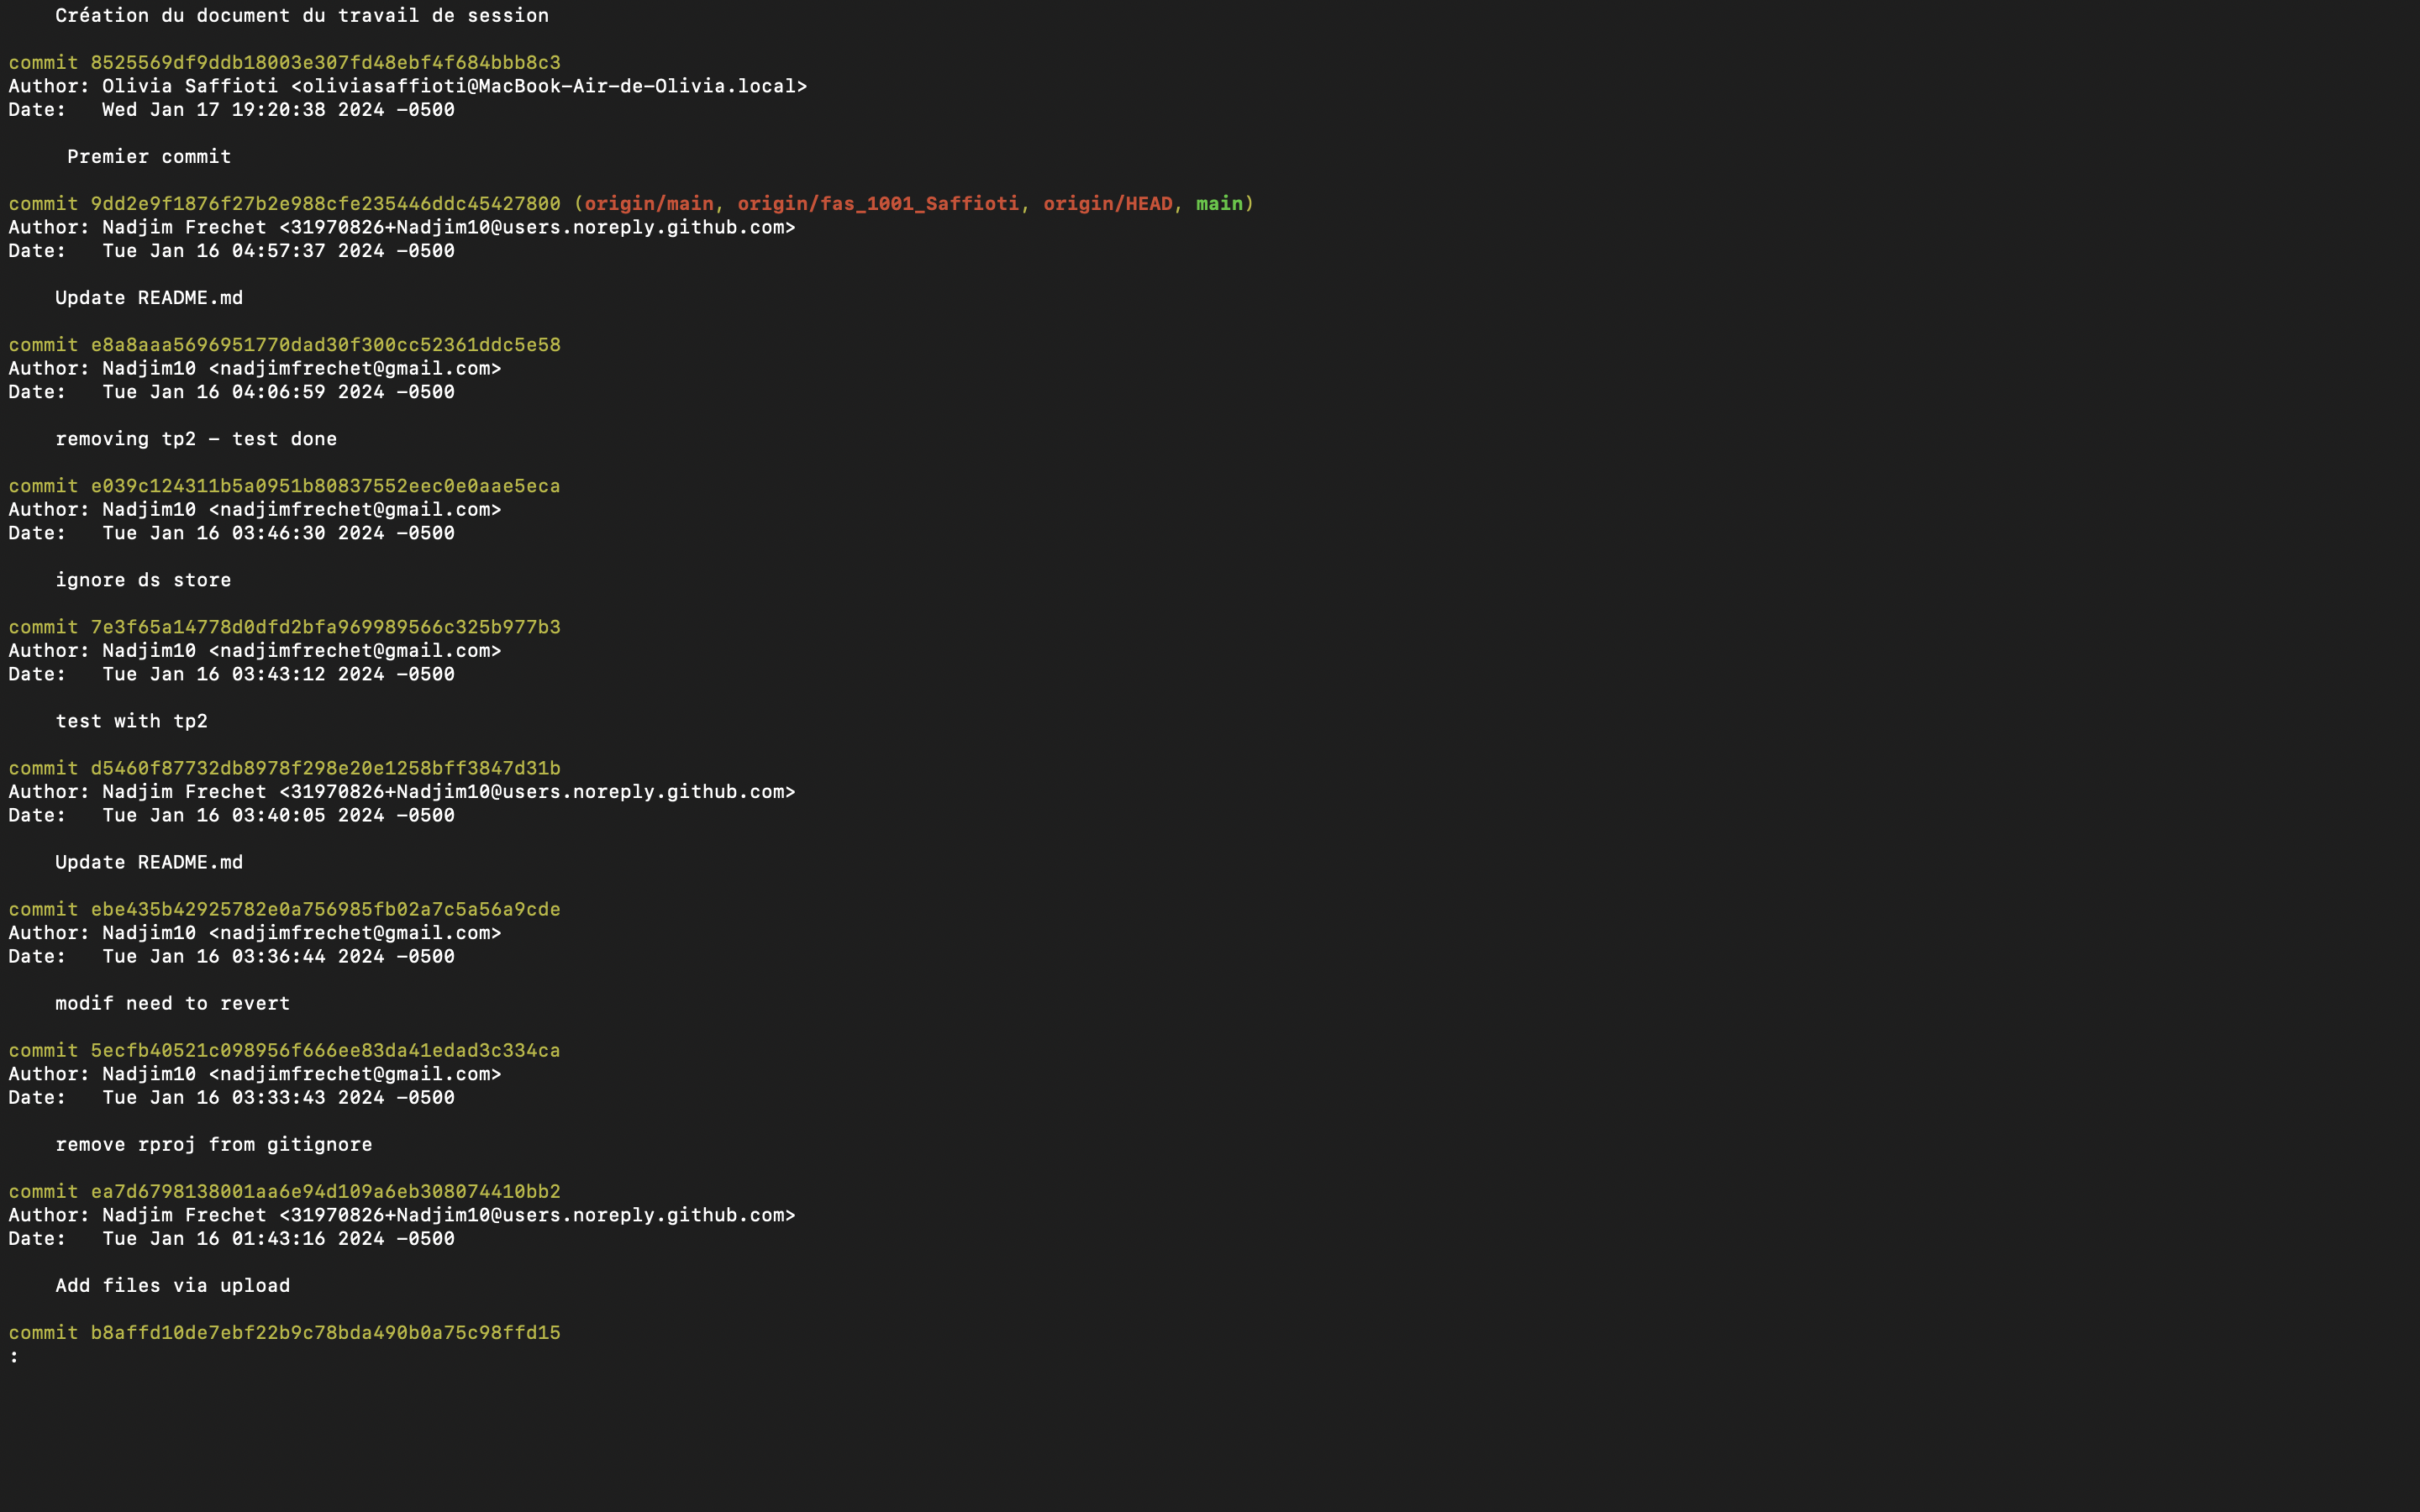
\includegraphics{//Users/oliviasaffioti/Desktop/fas_1001_Saffioti/_tp/Codes Git 3.png}
\#\# Étape 1 du TP :

\hypertarget{transfuxe9rer-le-fichier-de-github-uxe0-notre-ordinateur}{%
\subsubsection{Transférer le fichier de Github à notre
ordinateur}\label{transfuxe9rer-le-fichier-de-github-uxe0-notre-ordinateur}}

\hypertarget{cd-desktop}{%
\paragraph{cd desktop :}\label{cd-desktop}}

Pour installer le fichier présent dans Github sur notre ordinateur, nous
avons utilisé la commande ``cd desktop'' afin d'installer le fichier sur
notre bureau. Cette commande permet de déterminer un ``répertoire'' (ici
le bureau/desktop) dans lequel placer le fichier.

\hypertarget{git-init}{%
\paragraph{git init :}\label{git-init}}

Nous avons utilisé la commande ``git init'' afin de configurer notre
répertoire. Cette configuration a permis au répéertoire de devenir un
dépôt Git. De cette manière, il est devenu possible d'avoir un suivi des
versions de notre projet ou encore de gérer les branches et les commits.

\hypertarget{git-clone}{%
\paragraph{git clone :}\label{git-clone}}

Nous avons ensuite utilisé la commande ``git clone'' afin d'importer le
fichier sur notre ordinateur. Pour ce faire, nous avons copier coller le
lien Github du fichier à la suite de ce code. Cette commande a permis de
cloner le fichier présent sur Github.

\hypertarget{section}{%
\subsection{}\label{section}}

\hypertarget{renommer-le-fichier-importuxe9}{%
\subsubsection{Renommer le fichier
importé}\label{renommer-le-fichier-importuxe9}}

\hypertarget{mv-fas_1001-fas_1001_saffioti}{%
\paragraph{mv fas\_1001
fas\_1001\_Saffioti}\label{mv-fas_1001-fas_1001_saffioti}}

Afin de renommer notre fichier, nous avons utilisé la commande ``mv''
suivie de l'ancien nom du fichier et du nouveau nom que nous voulions
lui attribuer. Le fichier a ainsi été nommé ``fas\_1001\_Saffioti''.

\hypertarget{uxe9tape-2-du-tp}{%
\subsection{Étape 2 du TP :}\label{uxe9tape-2-du-tp}}

\hypertarget{cruxe9er-une-nouvelle-branche}{%
\subsubsection{Créer une nouvelle
branche}\label{cruxe9er-une-nouvelle-branche}}

\hypertarget{cd-fas_1001_saffioti}{%
\paragraph{cd fas\_1001\_Saffioti :}\label{cd-fas_1001_saffioti}}

Afin de créer une nouvelle branche, nous avons dans un premier temps
utilisé la commande ``cd'' suivi du nom de notre fichier pour accéder au
répertoire de notre projet.

\hypertarget{git-checkout--b-fas_1001_saffioti}{%
\paragraph{git checkout -b
fas\_1001\_Saffioti}\label{git-checkout--b-fas_1001_saffioti}}

Nous avons ensuite pu créer une nouvelle branche avec la commande ``git
checkout -b'' suivie du nom que nous voulions donner à la branche (ici :
fas\_1001\_Saffioti).

\hypertarget{uxe9tapes-4-et-6-du-tp}{%
\subsection{Étapes 4 et 6 du TP :}\label{uxe9tapes-4-et-6-du-tp}}

\hypertarget{ajouter-les-enregistrements-des-modifications-de-notre-fichier-dans-notre-historique-git}{%
\subsubsection{Ajouter les enregistrements des modifications de notre
fichier dans notre historique
Git}\label{ajouter-les-enregistrements-des-modifications-de-notre-fichier-dans-notre-historique-git}}

\hypertarget{git-add-.}{%
\paragraph{git add . :}\label{git-add-.}}

La commande ``git add .'' nous a permis d'ajouter les modifications de
notre fichier au sein de notre historique git et dans notre répertoire
de travail. Cette commande permet de faire un état des modifications
apportées au fichier, avant de les enregistrer au sein d'un commit.

\hypertarget{git-commit--m-premier-commit-et-git-commit--m-cruxe9ation-du-document-de-travail-de-session}{%
\paragraph{git commit -m ``Premier commit'' et git commit -m ``Création
du document de travail de session''
:}\label{git-commit--m-premier-commit-et-git-commit--m-cruxe9ation-du-document-de-travail-de-session}}

Nous avons utilisé la commande ``git commit -m'' suivie du ``nom que
nous souhaitions donné à notre commit'' (ici ``Premier commit'' et
``Création du document de travail de session''). Ce code nous a permis
de créer un commit avec les modifications que nous avons apporté à notre
fichier. Ce commit a pris en considération l'état de notre fichier, avec
les changements que nous y avons apporté. En somme, il a permis
l'enregistrement définitif des modifications du fichier.

\hypertarget{git-branch}{%
\paragraph{git branch :}\label{git-branch}}

Nous avons utilisé la commande ``git branch'' afin de vérifier que nos
commits étaient effectués au sein de la bonne branche (à savoir
fas\_1001\_Saffioti).

\hypertarget{uxe9tape-7-du-tp}{%
\subsection{Étape 7 du TP :}\label{uxe9tape-7-du-tp}}

\hypertarget{guxe9nuxe9rer-lhistorique-des-commits}{%
\subsubsection{Générer l'historique des
commits}\label{guxe9nuxe9rer-lhistorique-des-commits}}

\hypertarget{git-log}{%
\paragraph{git log :}\label{git-log}}

Nous avons utilisé la commande ``git log'' afin d'afficher une liste
détaillant les commits que nous avons générés. Ils sont affichés du plus
récent au plus ancien. L'auteur des commits, l'identifiant des commits,
la date et l'heure des commits, ainsi que le message des commits sont
exposés.



\end{document}
